\chapter{Known Slideshow Applications}
Apple Keynote and Microsoft PowerPoint are slideshow applications which use drag-and-drop functions, which is why these will not be focussed on further, because this approach to create slideshows does not fulfill the requirements of being a non-pointing device based application, as specified in the problem formulation \ref{ProblemFormulation} of this report. The main focus will be on the differences between \LaTeX~Beamer and the slideshow programming language, NISSE, developed in this project.

\section{\LaTeX~Beamer}
An example of \LaTeX~Beamer is listed in listing \ref{lst_beamer}.

\begin{lstlisting}[frame=single, caption={Beamer example}, label=lst_beamer]
%\textbf{Main\_document.tex}%
\begin{document}
\include{Slide_document.tex}
\end{document}

%\textbf{Slide\_document.tex}%
\frame {
	\frametitle{Welcome to this course}

This course will contain information about how you \underline{underline} things, and how you do other \textit{weight stuff} on sentences. \\
\textbf{{Like this}} \\	}
}
\end{lstlisting}

\begin{figure}[H]
	\centering
		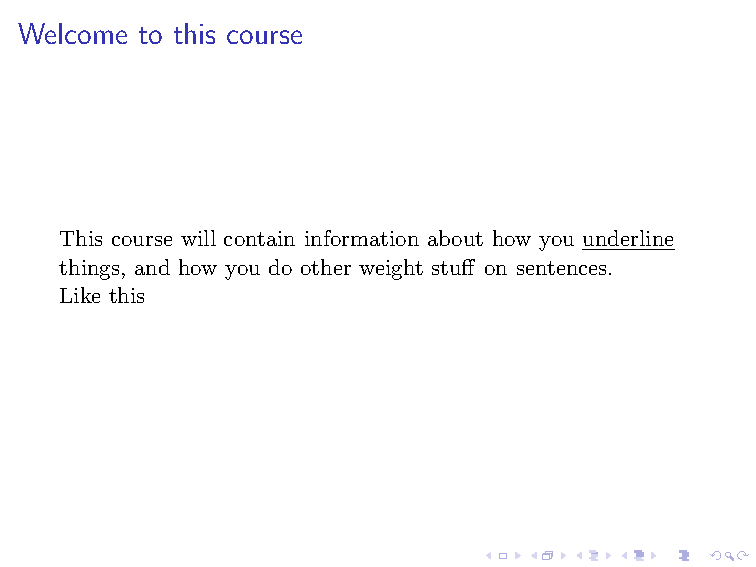
\includegraphics[width=0.8\textwidth]{text/beamer_example.pdf}
	\caption{\LaTeX~Beamer output}
	\label{fig:beamer_example}
\end{figure}

\noindent{The example seen in listing \ref{lst_beamer}, is a \LaTeX~Beamer-code example for expressing the output in figure \ref{fig:beamer_example}. The \LaTeX~Beamer-code seen in listing \ref{lst_beamer} is only to express the output shown. To make a slideshow using \LaTeX~Beamer you have to set up a main document. In this document, all settings about; theme, colours, inputs (other files), etc., for the slideshow is set up. \LaTeX~editors (e.g. TexMaker), only generates a very small amount of the main document, which leaves a lot of setup for the user, if additional settings is wanted. If only a general slideshow is required, the main document will not need much work. A general slideshow is without colours, themes or the need for additional packages.\\
Compared to the \LaTeX~Beamer-code the developed language should be made more compact to make slides faster to express.}
\\ \\
A test between \LaTeX~Beamer and the developed language will be made to determine which and why the one language is better suited for expressing slideshows than the other.
